\chapter[ASTHROS Payload Readout System Design]{ASTHROS Payload Readout System Design}
ASTHROS, the Astrophysics Stratospheric Telescope for High Spectral Resolution Observations at Submillimeter-wavelengths, is a balloon-borne observatory designed to study the universe in the submillimeter wavelength range.
The readout system is responsible for controlling the detectors, reading out the data, and storing the data on a solid state drive.
The readout system is designed to be modular and scalable, allowing for easy integration of new detectors and readout systems.
Each module is designed to be self-contained, focusing on a single device in the readout system so that changes to the hardware can be made without affecting the rest of the system.

\section{Network Architecture}
\subsection{Raspberry Pi Compute Module 4}
From a fresh install of Raspberry Pi OS, we need to install the necessary packages to run the readout system.
The first step is to enable Secure Shell (SSH) so that we can remotely access the Raspberry Pi.
This can be done in the Raspberry Pi Configuration tool by enabling SSH in the Interfaces tab.
While we're in the interfaces tool, we can also enable SPI and Remote GPIO. 
These are necessary to interface with the PMCC.

Next, we need to configure the networking interfaces. 
\texttt{eth0} is the wired interface to the rest of the readout network. 
We need a static IP for the CM4 to ensure that other devices on the network can easily find it.
In the network settings at the top right of the screen, we can select "Edit Connections" under Advanced Options. 
From there, you will see "Wired connection 1" which is the default name for the wired interface.
Select the interface and navigate to the IPv4 Settings tab.
Chance the method from "Automatic (DHCP)" to "Manual" and add the IP address, Netmask, and Gateway.
For ASTHROS, we have the IP addresses of all CM4s set to \texttt{192.168.1.13X} where \texttt{X} is uniquely assigned to each CM4.
The Netmask is set to \texttt{23} so we can access all devices on the \texttt{192.168.1.X} readout network as well as the \texttt{192.168.0.X} gondola network.
Finally, the Gateway is set to \texttt{192.168.1.1} when attached to the gondola and \texttt{192.168.1.101} when attached to the readout network.
This is because, when connected to a test bench, we utilize the NAS as our router to access other devices on the network.
When connected in flight configuration, we disable the NAS's router functionality and use the gondola's router instead.

Next, we need to configure the SPI interface to work with the PMCCs.
This process is different for Compute Module 5s (CM5s) as they have a different SPI driver and interfaces for the GPIO pins.
While we are in the process of upgrading to CM5s, the current version of the readout, and thus this documentation, is designed for CM4s.
The first step is to increase the SPI buffer size.
This is done by appending the following to the end of the \texttt{/boot/cmdline.txt} file:
\begin{verbatim}
    spidev.bufsiz=65536
\end{verbatim}
This sets the SPI buffer size to 64KB which is the maximum size to support the burst readout of the PMCCs.
For loading on boot, we need to add the SPI device to the \texttt{/etc/modules} file.
This is done by adding the following line to the file:
\begin{verbatim}
    spi_bcm2835
\end{verbatim}
Each of the CM4s will control up to four PMCCs, so we need to enable unique SPI busses for each PMCC.
This is done on the \texttt{/boot/config.txt} file by adding the following lines:
\begin{verbatim}
    dtoverlay=spi0-1cs
    dtoverlay=spi3-1cs
    dtoverlay=spi4-1cs
    dtoverlay=spi5-1cs
\end{verbatim}
This enables the SPI0, SPI3, SPI4, and SPI5 busses on the CM4.
While we could, in theory, only use two SPI busses and use the chip select lines to control two PMCCs on each bus, we decided to use a single chip select line for each PMCC to simplify the wiring harness and ensure our bandwidth is not saturated.

At this point, it is a good idea to reboot the CM4 to ensure that all changes have taken effect.
To verify the SPI busses are enabled, we check the \texttt{/dev} directory for the SPI devices which should be \texttt{/dev/spidevX.0} where \texttt{X} is the SPI bus number (0, 3, 4, or 5).
After rebooting and verifying the SPI has been set up, we recommend connecting the CM4 to the internet through a wireless hotspot in order to install the necessary libraries.
The first library we need to install is the pigpio.
This is a library that allows us to control the GPIO pins on the CM4 without needing root access.
To install the pigpio library, we need to run the following commands:
\begin{verbatim}
    sudo apt-get update
    sudo apt-get install pigpio
\end{verbatim}
After installing the pigpio library, we need to enable the pigpio daemon to run on boot.
This is done by running the following command:
\begin{verbatim}
    sudo systemctl enable pigpiod
\end{verbatim}

Finally, we need to install the actual Python packages that we will use to control the PMCC.
First we need to clone the \texttt{PyMCC} repository from GitHub.
This is done by running the following command:
\begin{verbatim}
    git clone https://github.com/asthros/pymcc.git
\end{verbatim}
Because this is a private repository, you will need to enter your GitHub username and personal access token.
You will need to generate a personal access token on GitHub and use that as your password when prompted.
After cloning the repository, we need to install the Python packages.
This is done by running the following command:
\begin{verbatim}
    pip3 install -r pymcc/requirements.txt
\end{verbatim}
This will install all the necessary packages to run the \texttt{PyMCC} package.

Finally, we need to edit the hosts file on the CM4 to ensure that we can access the other devices on the readout network by name.
This is done by updating the \texttt{/etc/hosts} file with the IP addresses and hostnames in Appendix \ref{chap2/appendix:hosts}.

\section{RabbitMQ and RMQTools}

\section{PMCC}
For ASTHROS, we utilize an array of 4GHz spectrometers called the PMCC ASIC P19800B ASIC RF Spectrometer, henceforth referred to as the PMCC.
These PMCCs are interfaced with via SPI for control, diagnostics, and readout \citep{PMCCP19800B}.
To communicate with the PMCCs, we utilize Raspberry Pi Compute Module 4s (CM4s) with custom harnesses.
The CM4 was chosen because it can be configured to operate at the 1.8V logic level necessary for PMCC by moving a diode on the CM4 IO board \citep{cm4io}.
Additionally, the CM4 has 4 SPI buses, allowing us to control up to 4 PMCCs per device \citep{cm4}.
The PMCCs are also connected to a GPIO pin on the CM4 to allow us to send a reset signal to the PMCCs.
The custom harness used to connect the PMCCs to the CM4 mounts onto the CM4 IO board's GPIO pins and converts the 40 ribbon cable to four sets of connections for the PMCC's SPI and reset pins.
Additionally, the CM4 has an SSD mounted to the side of it's IO board enclosure for raw spectra storage and easier local debugging when the device is not connected to the rest of the readout network.
Finally, two CM4s and eight PMCCs are mounted in a custom enclosure that is designed to be mounted on the back of the ASTHROS primary mirror.

\texttt{PyMCC} is the Python package developed to interface with the PMCCs and communicate with the rest of the readout system.
Originally, the PMCCs were controlled by a C program that was designed to provide a simple CLI for manually controlling the PMCCs.
As we needed to control multiple PMCCs and have them communicate with the rest of the readout system, we decided to rewrite the control software and drivers in Python.
The core of \texttt{PyMCC} is a Python driver for the PMCCs that provides an interface for controlling the PMCCs and reading out the data.
Built on top of the driver are Python programs that allow for manual control of the PMCCs, as well as a server that allows for control of the PMCCs over the RabbitMQ network.

\subsection{\texttt{spi\_utils}}
At the lowest level of the \texttt{PyMCC} driver is the \texttt{spi\_utils} module.
This module provides an interface for communicating with the PMCCs over SPI using the \texttt{spidev} Python library.
The \texttt{spidev} library provides an interface to the Linux kernel's SPI device driver \citep{spidev}.
Additionally, the PMCC has 16-bit registers that require us to send and receive 16-bit words instead of the typical 8-bit bytes that \texttt{spidev} expect. 
This was the primary reason for the development of the \texttt{spi\_utils} module as it handles the conversion between 16-bit words and 8-bit bytes and provides an easier interface for configuring the PMCCs registers without having to worry about the low-level details of the SPI communication.

The \texttt{spi\_utils} module provides a \texttt{PMCC\_SPI} class that is used to communicate with the PMCCs.
The \texttt{PMCC\_SPI} class is initialized with the bus, device, SPI mode, bits per word, and clock speed for the PMCC with which we are communicating.
The bus and device are specific to the PMCC we are communicating with and are based on the wiring harness used to connect the PMCC to the CM4.
The SPI mode, bits per word, and clock speed are all set to the values specified in the PMCC manual.

To simplify addresses, the \texttt{PMCC\_SPI} object has a \texttt{make\_addr()} method that takes the address of the register we want to write to and the read/write bit.
Valid addresses for the PMCC are 0-511, and the read/write bit is 0 for a write and 1 for a read.
When sending a command to the PMCC, the first word of the command is the address of the regster we want to write to shifted left by 1 bit to make room for the read/write bit.
\begin{equation}
    \text{tx[16]} = \text{addr[9]} << 1 + \text{rw[1]}
\end{equation}
Because \texttt{spidev} uses 8-bit communication, we need to split the 16-bit word into two 8-bit bytes.
\begin{equation}
    \label{chap2/eq:split_word}
    \text{byte[8][2]} = [\text{word[16]} >> 8,\ \text{word[16]}\ \text{\&}\ \text{0xFF}]
\end{equation}
The helper method returns these two bytes as an array that can be used in other methods to convert an address and command into a format that can be sent over SPI.

For reading and writing to the PMCC, the \texttt{PMCC\_SPI} object has an \texttt{xfer()} method that takes the address of the register, a read or write flag, and optional data to write and length of data to read.
By default, the length of data to read is 1, and the data to write is None.
The \texttt{xfer()} method first obtains the TX bytes from the \texttt{make\_addr()} method.
For both read and write commands, we utilize the \texttt{spidev} library's \texttt{xfer3()} function as it allows us to send and receive data of arbitrary length in a single SPI transaction \citep{spidev}.
\texttt{spidev}'s \texttt{xfer2()} and \texttt{xfer()} will fail at list values longer than the maximum SPI buffer size.
On the other hand, \texttt{xfer3()} will automatically split the data into multiple SPI transactions if the data is longer than the maximum SPI buffer size.
This is vital for burst reads on the PMCC as our data can be much longer than the maximum SPI buffer size.
For writes, the \texttt{xfer()} method sends the TX bytes and the data to write to the PMCC.
The data is split into two 8-bit bytes using Equation \ref{chap2/eq:split_word}.
During this transaction, the PMCC does not send any data back, so the \texttt{xfer3()} function returns an array of zeros.
If our transaction is unsuccessful, instead of returning zeroes, we will receive an empty array that we can check for.
For single register reads, the \texttt{xfer()} method sends the TX bytes followed by a dummy word to the PMCC.
While we are sending the dummy word over the MOSI line, the PMCC is sending the data we requested over the MISO line that is returned by the \texttt{xfer3()} function along with the original TX bytes.
After checking that we have received data from the PMCC, we return the data as an array of 16-bit words.
This is done by utilizing NumPy to cast the output as a \texttt{np.uint8} array and then returning a view of that array with big-endian 16-bit unsigned integer data type \citep{numpy}.
For reads that are longer than a single register, we send the TX bytes followed by a dummy word for each word we want to read and follow the same process as a single register read.

For simple reads, \texttt{PMCC\_SPI} has a \texttt{read()} method that takes the address of the register we want to read from and optionally the number of words we want to read.
By default, this method reads a single word from the PMCC.
The \texttt{read()} method calls the \texttt{xfer()} method with the read flag set to 1 and the number of words to read.
If we are only reading a single word, we return the first word and only word in the array of words returned by the \texttt{xfer()} method. 
Otherwise, for burst reads, we return the entire array of words.

Often times, we want to read a specific value over and over until that value is True.
Many status bits on the PMCC operate in this way to indicate when a specific operation has completed. 
To accomplish this, the \texttt{PMCC\_SPI} object has a \texttt{poll()} method that takes the address of the register we want to read from, the bit within the register we want to check, the amount of time to wait between reads, and the maximum number of reads.
The \texttt{poll()} method then issues a \texttt{read()} of that register and checks if the bit is set by shifting the read value to the right by the bit number and checking if the least significant bit is set.
If the value is not set, we wait for the specified amount of time and read the register again.
This process is repeated until the value is set or the maximum number of reads is reached.
We then return if the value was set or not instead of raising an exception if the value is not set.
The implementation of raising exceptions is left to the user of the \texttt{poll()} method depending on the use case.

For simple writes, \texttt{PMCC\_SPI} has a \texttt{write()} method that takes the address of the register we want to write to and the data we want to write.
The \texttt{write()} method calls the \texttt{xfer()} method with the read flag set to 0.
From there, the \texttt{xfer()} method sends the data to the PMCC and returns None as the PMCC does not send any data back.
If there is an issue with the transaction, the \texttt{xfer()} method will raise an exception indicating that it received null from the transfer to the specific address. 

The documentation for the PMCC specifies specific bits and ranges of bits within a register address to set different configurations on the device.
We often only want to change a specific value at an address and not the entire register.
To accomplish this, the \texttt{PMCC\_SPI} object has a \texttt{mask\_data()} method that takes the most significant bit (MSB), the least significant bit (LSB), the value we want to write, and the original buffer we are overwriting.
This closely matches the way the PMCC documents the use of each register with either a single bit or an inclusive range of bits. 
First we check if the MSB and LSB are valid values, and if they are not, we raise an exception.
Valid values for addressing the 16-bit registers are 0 to 15 for the LSB and LSB to 15 for the MSB.
Next, we check if the value provided will fit within the length specific by the MSB and LSB.
We then use the MSB and LSB to calculate the maximum value that will fit in the mask. 
We use this maximum value to determine if the provided value is too large, in order to raise an exception if it is.
Finally, we create a mask using the maximum value and shifting it to the left by the LSB.
We then take the original buffer and do a bitwise AND with the inverse of the mask to clear the bits between the LSB and the MSB. 
Finally, we shift our data to the left by the LSB and do a bitwise OR with the original buffer to set the bits between the LSB and MSB to the new value.
This process is shown in Equation \ref{chap2/eq:mask_data}.
\begin{align}
    \label{chap2/eq:mask_data}
    \text{maxValue} &= (1 << (\text{MSB} - \text{LSB} + 1)) - 1 & 0 \leq \text{LSB} \leq \text{MSB} \leq 15\\
    \text{mask} &= \text{maxValue} << \text{LSB} \\
    \text{buffer} &= (\text{buffer}\ \&\ \sim\text{mask})\ |\ (\text{data} << \text{LSB}) & 0 \leq \text{data} \leq \text{maxValue}
\end{align}

To further simplify the process of setting specific bits in a register, the \texttt{PMCC\_SPI} object has a \texttt{read\_write()} that first reads from the address we want to write to, modifies the data we want to change, and then writes the modified data back to the PMCC.
The \texttt{read\_write()} method takes the address of the register we want to read from and one of the following formats for the data we want to write:
\begin{itemize}
    \item A tuple of MSB, LSB, and value to write to the register 
    \begin{itemize}
        \item e.g. \texttt{(15, 8, 0xAA)} would set the register to \texttt{0b1010 1010 XXXX XXXX}
    \end{itemize}
    \item A tuple of a single bit and value to write to the registers
    \begin{itemize}
        \item e.g. \texttt{(2, 0x1)} would set the register to \texttt{0bXXXX XXXX XXXX X1XX}
    \end{itemize}
    \item An array containing combinations of the above two formats
    \begin{itemize}
        \item e.g. \texttt{[(15, 8, 0xAA), (2, 0x1)]} would set the register to \texttt{0b1010 1010 XXXX X1XX}
    \end{itemize}
\end{itemize}
The \texttt{read\_write()} method first reads the data from the PMCC using the \texttt{read()} method and stores it in a buffer.
Then we check if the changes provided are a tuple or an array of tuples.
If it's a tuple, we just wrap it in an array in order to iterate over it.
For each change in the array, we unpack the tuple and call the \texttt{mask\_data()} method to modify the data we read from the PMCC, updating the buffer each time.
If we are only changing a single bit, MSB and LSB are set to the same value.
To complete the transaction, we write the modified buffer back to the PMCC using the \texttt{write()} method.


Finally, we provide a \texttt{close()} method that simply calls the \texttt{close()} method on the \texttt{spidev} object to close the SPI connection.

\subsection{\texttt{config}}
There are a number of device specific configurations that need to be set for each PMCC in order to operate correctly.
To simplify the process of writing code to configure the PMCCs, we utilize the YAML configuration file format to store the configuration for each PMCC \citep{yaml}.
This YAML file has information about the RMQ configuration as well as spectrometer configuration. 
For now, we will focus on the spectrometer configuration and discuss the RMQ configuration in Section \ref{chap2/section:rmqtools}.
The spectrometer config section, \texttt{spec}, is split into two main sections for the PMCCs, global variables used for every spectrometer, and spectrometer specific variables.
For each experiment, we would like to have a single configuration file that can be used on every CM4 to configure multiple PMCCs. 
To accomplish this, each CM4 is given a unique name that we use to differentiate between each device. 
Each PMCC connected to a CM4 is then indexed, so we can individually address each one by specifying the CM4 name and the PMCC index.

The format for the global configurations is shown in Table \ref{chap2/table:pmcc_config}.
These configurations are used to set values we don't expect to individually change for each PMCC.
While we may create different configurations for different experiments, such as integration time and magnitude or power mode, we will likely make these changes to all PMCCs at once and not individually.

\begin{table}[h!]
    \centering
    \begin{tabularx}{\textwidth}{l|l|X}
        \textbf{Key} & \textbf{Type} & \textbf{Description} \\ \hline    
        \texttt{spec\_file} & path & Path to the spectrometer hardware file \\
        \texttt{int\_time} & int & Integration time in milliseconds \\
        \texttt{clock\_freq} & int & Reference clock frequency in MHz \\
        \texttt{resolution} & int & 16 or 32 for 16-bit or 32-bit readout resolution \\
        \texttt{shift} & int & 0 or 4 for 0 or 4 bit shift \\
        \texttt{magnitude} & bool & True for magnitude mode, False for power mode \\
        \texttt{window\_bypass} & bool & True to enable rectangular window bypass \\
        \texttt{window\_bit\_growth} & bool & True to enable window div 2 bypass \\
        \texttt{butterfly\_shift} & bool & True to enable butterfly shift for improved noise measurements \\
        \texttt{wiring} & array & See Table \ref{chap2/table:wiring} for wiring configuration \\
        \texttt{groups} & dict & Dictionary of CM4 names and an array of PMCC chip IDs  \\
    \end{tabularx}
    \label{chap2/table:pmcc_config}
    \caption{Global Variables in the PMCC Configuration File}
\end{table}

After the global configurations, an array of four spectrometer wiring configurations is provided. 
In full operation, we will have four PMCCs connected to each CM4, so we need a way of specifying the wiring for each PMCC's SPI bus and GPIO reset pin.
Because the harness is identical for each CM4, we can specify the wiring for each PMCC along the harness, and it will be the same for every CM4. 
The only exception to this is the lone 100GHz PMCC connected to its own CM4. 
The wiring for this PMCC is simply the first index in the wiring array will still work with the rest of the system.
Each item in the wiring configuration is as follows in Table \ref{chap2/table:wiring}.

\begin{table}[h!]
    \centering
    \begin{tabularx}{\textwidth}{l|l|X}
        \textbf{Key} & \textbf{Type} & \textbf{Description} \\ \hline    
        \texttt{dev} & string & Path to device address (e.g. \texttt{/dev/spidev0.0}) \\
        \texttt{gpio} & int & GPIO pin number for the reset signal\\
        \texttt{speed} & int & SPI device speed in Hz, typically 5000000 unless changes for stability reasons and debugging\\
    \end{tabularx}
    \label{chap2/table:wiring}
    \caption{Wiring Configuration in the PMCC Configuration File}
\end{table}

Finally, we have the group configuration dictionary. 
Each PMCC comes with a chip ID specified by the manufacturer used to set pre-calibrated values, such as the ADC time skew.
The configuration dictionary consists of a CM4 name as the key and an array of PMCC chip IDs as the value.
This allows us to specify which PMCCs are connected to each CM4 and configure them accordingly.
For the 100GHz PMCC and CM4, the array will only contain a single chip ID.

When loading in the configuration file, we create a \texttt{PMCC\_Config} object that all configuration information necessary for the CM4. 
We initialize this object with the \texttt{spec} part of the YAML file, the group name of the CM4, and an array of PMCC indexes to configure (e.g. \texttt{[1, 2, 3, 4]} for all spectrometers).
The \texttt{PMCC\_Config} object then creates properties for each of the global configurations that can be accessed by the \texttt{PMCC\_SPI} object.
We set the resolution mode of the PMCCs using the \texttt{resolution} and \texttt{shift} properties and a lookup table for the proper register values as shown in Table \ref{chap2/table:resolution}.
We could, theoretically, set higher values for LSB shift but for the purposes of ASTHROS, we only need 0 and 4 bit shifts.

\begin{table}
    \centering
    \setlength{\extrarowheight}{2pt}
    \begin{tabular}{cc|c|c|}
      & \multicolumn{1}{c}{} & \multicolumn{2}{c}{Resolution}\\
      & \multicolumn{1}{c}{} & \multicolumn{1}{c}{\texttt{16-Bit}}  & \multicolumn{1}{c}{\texttt{32-Bit}} \\\cline{3-4}
      \multirow{2}*{LSB Shift}  & $0$ & \texttt{0x080} & \texttt{0x0C0} \\\cline{3-4}
      & $4$ & \texttt{0x180} & \texttt{0x1C0} \\\cline{3-4}
    \end{tabular}
    \caption{Resolution Mode Configuration for PMCC}
    \label{chap2/table:resolution}
\end{table}

After the global variables are loaded, we create a dictionary of device configurations for individual PMCCs. 
This dictionary is indexed by the CM4 group name concatenated with the PMCC index.
Each value in the dictionary is a \texttt{PMCC\_Device\_Config} object that is initialized with the chip ID, the wiring configuration at the PMCC index, and the \texttt{spec\_file} for configuration.
The wiring information is paired with the chip ID to create a \texttt{PMCC\_Device\_Config} object that can later be used to configure the PMCC. 
The provided \texttt{dev} path for the SPI configuration is split and stored into the bus and device number for the \texttt{PMCC\_SPI} object to use.
Finally, the pre-calibrated values are loaded from the \texttt{spec\_file} by searching for the chip ID in the file and storing the associated values in the \texttt{PMCC\_Device\_Config} object.
If the chip is not found in the file, we raise an exception that the configuration provided was not valid. 
The final product is a \texttt{PMCC\_Config} object that contains all the necessary information to configure both the CM4 and any number of PMCCs connected to it. 

\subsection{\texttt{consts}}
The \texttt{consts} module is simply a collection of constants used throughout the \texttt{PyMCC} module.
Many of these are register addresses so that we can easily reference them in the code without having to go back and forth between the PMCC manual and the code.
Additionally, we have some large arrays that are used in configuration that we don't want to hard code into the code.
For example, \texttt{WINDOW\_COEFFS} is a vector of 513 values used to configure the symmetrical 1024 point FFT on the DSP. 
In addition to addresses and coefficients, we keep an array of default values for the PMCC registers so that we can easily identify issues with the device after reset. 

\subsection{\texttt{driver}}
The \texttt{driver} module is the highest level of the \texttt{PyMCC} package and is responsible for providing all functionality for the PMCCs. 
Each PMCC is controlled by a \texttt{PMCC\_Driver} object that is initialized with a \texttt{PMCC\_Config} object and the index of the spectrometer in the config that we want to control.
After initializing the object, the user must call the \texttt{initialize\_interface()} method to set up a \texttt{PMCC\_SPI} object to communicate with the PMCC.
Following SPI set up, the user must call the \texttt{initalize\_gpio()} method to set up the GPIO pin for the reset signal.
Both of these methods check the wiring configuration in the \texttt{PMCC\_Config} object to ensure that the correct wiring is provided.
With both of these methods called, the \texttt{PMCC\_Driver} object is ready to start the PMCC configuration. 

The first thing done before any configuration is toggling the reset signal on the PMCC.
This is done by calling the \texttt{reset()} method with a boolean value to set the reset signal high followed by low.
\texttt{reset()} is often called multiple times in the configuration process to ensure that the PMCC is in a known state before configuring it.

\begin{quote}
    \textbf{Note:} The PMCC documentation specifies individual bit fields for each register. 
    When referring to a specific register in the documentation, we will use the format \texttt{reg\_name} with lowercase letters. 
    These will be identical to the register names in the documentation. 
    During the development of \texttt{PyMCC}, we often had to refer to SPI addresses that contain multiple PMCC registers. 
    When referring to these addresses, we will use the format \texttt{REG\_NAME} with all uppercase letters.
    These are not documented in the PMCC manual but are used to reference addresses defined in the \texttt{consts} module.
\end{quote}

After resetting the PMCC, we need to calibrate the Phase Lock Loop (PLL) on the PMCC using \texttt{initialize\_pll()}.
The PLL is used to synthesize all required clocks for the PMCC with the use of an external reference clock. 
Initializing the PLL is done in three steps, resetting the PLL with \texttt{reset\_pll()}, calibrating the PLL with \texttt{calibrate\_pll()}, and finally loading the ADC with the PLL values using \texttt{load\_adc()}.
\texttt{reset\_pll()} resets the PLL and sets the ADC gain, offset, and time skew configurations. 
This is done by the following sequence of commands:

\begin{enumerate}
    \item 
        Write to the \texttt{CHIP\_CONF} to reset the DSP.
    \item 
        Read and write the \texttt{PLL\_LOCK\_CONF} to set the \texttt{lock\_desired\_count} to 3, \texttt{lock\_tune\_off} to 2, and \texttt{lock\_tune\_on} to 4. 
        These set the lock detector control that will later be used to determine if we have locked the PLL.
    \item 
        Read and write the \texttt{PLL\_FVCO\_CAL\_CONF} to set the \texttt{fvco\_cal\_settletime} to 4. 
        This is used by the PLL's Voltage Controlled Oscillator (VCO) to determine the settling time for the VCO.
        By setting this to 4, we are setting our settle time to $2^{4} = 16$ times the reference frequency.
    \item 
        Read and write the \texttt{ADC\_GAIN\_ACCUM} and set the \texttt{adc\_gain\_cal\_accum} to 3 which sets the on-chip gain calibration accumulator length to 8192. 
    \item 
        Read and write the \texttt{ADC\_GAIN\_CONF} and set the \texttt{adc\_gain\_cal\_settle} to 3 which adjusts the delay during the gain calibration to 63 clock cycles. 
    \item 
        Read and write the \texttt{ADC\_OFFS\_CONF} and set the \texttt{adc\_offs\_cal\_accum} to 3 and the \texttt{adc\_offs\_plr} to 1. 
        This sets the on-chip offset calibration accumulator length to 8192 and the polarity of the offset calibration to fine (comparator) adjustment mode. 
    \item 
        Read and write the \texttt{ADC\_TIME\_SKEW\_COEF} to set the \texttt{time\_skew\_select} to 0xF. 
        This enables the use of manual time skew codes for the ADC.
    \item 
        Finally, write to the \texttt{DEMUX\_DEL\_ADJ\_A} to \texttt{DEMUX\_DEL\_ADJ\_D} to adjust the delay in the input interleaver clock for the four ADC groups. 
        This value is set to 11 for all four registers, setting the delay to $18.8*11 = 206.8$ ps. 
        Currently, this step is hard coded to 206.8 ps but, in the future, we may want to adjust this value based on the chip ID as these values are pre-calibrated for each chip.
\end{enumerate}

After resetting the PLL, we calibrate the PLL using \texttt{calibrate\_pll()}.
This takes many of the values we set in \texttt{reset\_pll()} to execute the calibration process. 
The calibration process is as follows:

\begin{enumerate}
    \item 
        Check if the clock frequency set in the configuration is a multiple of 2000. 
        Clocks must be a factor of 2GHz to ensure that the PLL can lock to the reference clock.
    \item 
        Read and write to the \texttt{PLL\_CONF} and set the \texttt{pll\_freq\_adjust} and the \texttt{pll\_ndiv}. 
        The \texttt{pll\_freq\_adjust} is used to set the sampling rate of the ADC. 
        We set this value to 2 which indicates a 4GHz clock for the ADC. 
        The \texttt{pll\_ndiv} is used to set the divider ratio for the PLL feedback. 
        This value is calculated using $N_{div} = 2000 \text{MHz} / F_{freq}$ and set in the \texttt{pll\_ndiv} register. 
        For our 100 MHz reference clock, we set the \texttt{pll\_ndiv} to 20.
    \item 
        Now we begin the calibration process by reading and writing to the \texttt{PLL\_FVCO\_CAL\_CONF} to set the \texttt{fvc\_cal\_start} to 1 and resetting the \texttt{fvco\_cal\_settletime} to 4. 
        This starts the calibration process and sets the settling time to 16 times the reference frequency.
    \item 
        Finally, we poll the \texttt{fvco\_cal\_cal\_done} bit until the band selection is completed. 
        If the calibration is not completed after a default of 10 retries, we raise an exception indicating that the PLL calibration failed.
\end{enumerate}

After the PLL is calibrated, we load the ADC with the PLL values using \texttt{load\_adc()}.
Many of the commands sent during this set are writes instead of reads and writes.
This is because we actually want to override the registers are not setting to 0.
The process for loading the ADC is as follows:
\begin{enumerate}
    \item 
        Write to the \texttt{VGA\_CURRENT\_CONF} to set the \texttt{vga\_current\_out\_adjust} and \texttt{vga\_offset\_rng}.
        The \texttt{vga\_current\_out\_adjust} is used to adjust the reference current at the VGA output buffer from 2.1 to 6.3 mA in steps of .6 mA.
        We set this to $2.1 + 6 * .6 = 5.7$ mA by setting the value to 6.
        The \texttt{vga\_offset\_rng} is used to adjust the offset compensation reference current from 250 to 600 uA in steps of 50 uA.
        We set this value to $250 + 7 * 50 = 600$ uA by setting the value to 7.
    \item 
        Write to the \texttt{VGA\_GAIN\_CONF} to set the \texttt{vga\_peak\_cntrl} and \texttt{vga\_gain\_adjust}.
        The \texttt{vga\_peak\_cntrl} is used to reduce the inductive AC peak of the VGA by increasing the capacitance.
        We set this value to a code of 5.
        The \texttt{vga\_gain\_adjust} is used to adjust the VGA gain from 0 to 10.4 dB in steps of approximately .53 dB.
        We set this value to $8 * .53 = 4.24$ dB by setting the value to 8.
    \item 
        Write to the \texttt{VGA\_CONFIG} to enable the common-mode compensation (\texttt{vga\_cm\_comp}), the VGA offset compensation (\texttt{vga\_offset}), and the VGA enable (\texttt{vga\_en}).
        These values are all defaulted to enabled, but it is good practice to set them to ensure that the VGA is properly configured.
    \item 
        Write the four \texttt{adc\_time\_skew\_adjust1} to \texttt{adc\_time\_skew\_adjust4} registers to set the time skew for the ADC.
        These values are pre-calibrated for each chip and are set in the \texttt{PMCC\_Device\_Config} object.
    \item 
        Write to the \texttt{ADC\_TIME\_SKEW\_CONF} to set the \texttt{time\_skew\_mode}, \texttt{time\_skew\_select} and \texttt{time\_skew\_polarity}.
        The \texttt{time\_skew\_mode} is set to 1 to enable calibration for a configured time instead of continuous calibration.
        The \texttt{time\_skew\_select} is set to 0b1111 to enable each of the four time skew adjustments.
        The \texttt{time\_skew\_polarity} is set to 1 to enable inverse polarity of the time skew code adjustment direction.
    \item 
        Write a 0 to \texttt{adc\_rst\_n} to register a reset to the ADC.
    \item 
        Write a 0 to \texttt{adc\_sub\_clk\_gen\_rst\_n} to reset the clock generators for all four ADC groups.
    \item 
        Sleep for 100 ms to allow the ADC to reset.
    \item 
        Write a 1 to \texttt{adc\_rst\_n} to enable the ADC.
    \item 
        Write a 1 to \texttt{adc\_sub\_clk\_gen\_rst\_n} to enable the clock generators for all four ADC groups.
\end{enumerate}

After those three steps, the PLL is calibrated and the ADC is ready for configuration.
To verify this, the \texttt{PMCC\_Driver} object has a \texttt{check\_connection()} method that checks if we can read from the PMCC.
We first read the \texttt{CHIP\_ID} register to ensure that we can communicate with the PMCC.
Despite having the same name as the chip ID we use to differentiate between PMCCs, the \texttt{CHIP\_ID} register is a fixed value that is set by the manufacturer and will always be 0x6 for the second generation 4GHz PMCCs.
Reading the \texttt{CHIP\_ID} register is a good way to verify that SPI connection is working.
We then read the \texttt{PLL\_LOCK\_LOL} register to determine if we have a Loss of Lock (LOL) on the PLL.
If the PLL is locked, the \texttt{PLL\_LOCK\_LOL} register will be 0.
If we make it past both of these checks, we return True to indicate that the PMCC is connected and the PLL is locked.

The usual next step in the configuration process is to calibrate the gain and offset of the ADC. 
This is done by calling the \texttt{calibrate\_adc()} method.
This method is a wrapper for the \texttt{calibrate\_adc\_offset()} and \texttt{calibrate\_adc\_gain()} methods and runs both of them twice.
The calibrations run in interactive mode so running them twice allows the PMCC to iterate on the calibration values and get a more accurate result.
To run the offset calibration, we set the following values within the \texttt{ADC\_OFFS\_CONF} register:

\begin{itemize}
    \item \texttt{adc\_offs\_cal\_en} to 1 to enable the offset calibration
    \item \texttt{adc\_offs\_cal\_mode} to 1, setting the operation mode to a zero offset calibration.
    \item \texttt{adc\_offs\_cal\_interactive} to 1 to start a new calibration using the previous adjustment codes. 
\end{itemize}

After setting these values, we poll the \texttt{adc\_offs\_cal\_ack} bit until the calibration is complete.
For the gain calibration, we simply have to set the \texttt{adc\_gain\_cal\_en} to 1 to enable the gain calibration.
We then poll the \texttt{adc\_gain\_cal\_ack} bit until the calibration is complete. 
After both calibrations are run twice, we are done calibrating the ADC. 

In the instance we already know the values we want to set for the gain and offset, we provide a \texttt{calibrate\_adc\_preset()} method that takes arrays of the 23 gain and 23 offset values to set the calibration values.
These values are loaded into the 23 \texttt{ADC\_REF\_ADJUST\_XX} and 23 \texttt{ADC\_OFFS\_ADJUST\_COMP\_XX} registers respectively.
The \texttt{adc\_gain\_cal\_mode} and \texttt{adc\_offs\_cal\_mode} registers also need to bet set to 0x1 and 0x2 to enable the use of the preset values.

After calibrating the ADC, we are able to configure the DSP. 
This is highly subjective to the experiment being run but, for ASTHROS, we have a specific configuration that we use that works for the integration time and resolution we are using. 
In future version of the code, we will likely pull out some of the hard coded values and make them configurable in the YAML file.
The configuration process is as follows:
\begin{enumerate}
    \item Reset the DSP by writing a 1 to the \texttt{CHIP\_CONF} register's \texttt{dsp\_reset}.
    \item Load the window coefficients into the DSP by writing the 513 values in the \texttt{WINDOW\_COEFFS} array to the \texttt{WINDOW\_REGISTER} register one at a time followed by a pulse to the \texttt{dsp\_coeff\_dest\_wind} bit to shift store the value and shift the register.
    \item 
        Write to the \texttt{dsp\_skip\_fft\_stage} register to 0 to use all four stages of the FFT. 
        This results in 512 frequency bins per sub-band. 
    \item 
        Write to the \texttt{DSP\_READOUT\_CONF} with the mode from the configuration file as shown in Table \ref{chap2/table:resolution}. 
        This sets the resolution and shift for the readout.
    \item 
        Write to the \texttt{CHIP\_CONF} register to set the \texttt{dsp\_enable} bit to 1 to enable the DSP and \texttt{dsp\_acc\_mode} to 1 to enable continuous FFT operation. 
    \item 
        Read and write to the \texttt{FFT\_CONFIG} to set the \texttt{dsp\_magn\_bypass}, \texttt{dsp\_wind\_bypass}, \texttt{dsp\_div\_red\_wind}. 
        These values are set in the configuration file and are used to enable the magnitude or power mode, the windowing function, and window bit growth. 
    \item 
        Calculate the number of integrations to run based on the integration time. 
        We do this by diving our desired integration time by the length of time it takes to run a single accumulation on the DSP. 
        For the ADC running at 8 GS/s (Gigasamples per second) reading 16384 time domain bins, this number is 2.048 us.
        The number of accumulations we collect per integration is a 24-bit value split across two registers. 
        The 16 most significant bits are stored in the \texttt{dsp\_acc\_num\_msb} register and the 8 least significant bits are stored in the \texttt{dsp\_acc\_num\_lsb} register.
    \item 
        If we are in power accumulation mode, we need to set the data shift for the DSP. 
        The maximum output resolution is <40 bits so we need to shift the data to the right depending on the integration time.
        We calculate this by taking the binary logarithm of the number of accumulations per integration and subtracting 8.
        We get eight because there is a maximum output resolution of 40 bits and the most we can shift the value is 32.
        By subtracting 8 from the binary logarithm, we get the number of bits we need to shift the data to the right that would maximize the output resolution without overflowing the readout.
        This value is then stored in the \texttt{dsp\_data\_shift} register.
    \item 
        If we are using a butterfly shift, we set the data divide by 2 blocks to the following values:
        \begin{itemize}
            \item \texttt{dsp\_bfly\_shift\_pfb} to \texttt{0b10101} to alternate between enabled and disabled IFFT processor stages. 
            \item \texttt{dsp\_bfly\_shift\_fft} to \texttt{0b1010101010} to alternate between enabled and disabled FFT processor stages.
        \end{itemize}
        The combination of these essentially skips every other stage of the IFFT and FFT processor, increasing performance for band-limited noise measurements.
        It accomplishes this by skipping the stages that would divide the data by 2 to reduce the risk of overflow. 
    \item 
        Write to the \texttt{VGA\_CURRENT\_CONF} to set the \texttt{vga\_current\_out\_adjust} and \texttt{vga\_offset\_rng}.
        We set these values to the same values as we did in the ADC calibration.
    \item 
        Finally, we perform a \texttt{check\_connection()} to ensure everything is in order and return the status.
\end{enumerate}

At this point, the PLL has been locked, the ADC has been calibrated and the DSP has been configured. 
The most common next step is to start the DSP and begin acquiring data. 
This is done in two parts, pulsing the accumulation bit and then reading the data. 
Pulsing the accumulation bit is done in the \texttt{pulse\_acquisition()} method by writing a 1 to the \texttt{dsp\_start\_acc} register.
This starts the DSP's operation and begins accumulating data.
After starting accumulation, we immediately perform a single \texttt{retrieve\_data()} to clear any garbage data that may be present in the DSP's output buffer.

The \texttt{retrieve\_data()} method follows the following process to read a spectra from the DSP:
\begin{enumerate}
    \item 
        Read the \texttt{dsp\_data\_ready} register to determine if the DSP has finished accumulating data.
        We poll this register at a rate of 500 Hz for a maximum of 2000 retries. 
        Both of these values are adjustable agruments to this method but are set to 500 Hz and 2000 retries by default.
        If we don't recieve data after the maximum number of retries, we raise an exception indicating that the DSP did not finish accumulating data.
        Otherwise, we continue to the next step.
    \item 
        Write a pulse to the \texttt{dsp\_start\_readout} register to start the readout process. 
    \item  
        Take a timestamp to record the time the readout started.
    \item 
        Start the readout process by performing a burst read of the \texttt{DSP\_READOUT\_ADDRESS} at \texttt{0x4000}. 
        If we are performing a 32-bit readout, we read the address 8193 times to get the first half of our data. 
        Otherwise, for a 16-bit readout, we read the address 8192 times.
    \item 
        If we are performing a 32-bit readout, we read the second half of the data by reading the \texttt{DSP\_READOUT\_ADDRESS} at \texttt{0x8000} 8191 times.
        This strange number of reads is due to a bug that causes issues if reading two 8192 blocks of data.
        Without following this specific sequence, we will be missing one value in the second half of the data, shifting the entire readout. 
    \item 
        Regardless of the resolution, we write a pulse to the \texttt{dsp\_reset\_ready} register to begin the next accumulation.
        This discards any data that may be present in the readout buffer so that new data can be stored. 
    \item 
        Finally, we return the data and the timestamp to the user. 
        If the resolution is 32-bit, we concatenate the two arrays and use NumPy to return a view of the data as an array of 32-bit unsigned integers.
        Otherwise, for 16-bit readouts, we use NumPy to return a view of the data as an array of 16-bit unsigned integers.
\end{enumerate}

Another common operation after set up is to read raw data from the ADC. 
This can be useful to ensure that the ADC is working correctly by measuring the mean and swing of the digitized signal. 
The \texttt{retrieve\_adc()} method does just this using the following procedure. 
\begin{enumerate}
    \item Write a 0 to the \texttt{dsp\_reset} register and a 1 to the \texttt{dsp\_enable} to enable the DSP.
    \item Write a 0 to the \texttt{dsp\_proto\_en} to disable prototype mode on the ADC.
    \item Write a 0 to the \texttt{DSP\_DEBUG\_MODES} to clear any other debug modes that may be enabled.
    \item Write a 1 to the \texttt{debug\_wr\_from\_adc} register at the \texttt{DSP\_DEBUG\_MODES} address to begin writing ADC samples into the debug buffer. 
    \item Begin polling the \texttt{debug\_wr\_from\_adc\_done} register to determine when the ADC samples have been written to the debug buffer. If we reach the maximum number of retries, we raise an exception that the ADC data was not ready after the maximum number of retries.
    \item Write a 0 to the \texttt{DSP\_DEBUG\_MODES} to disable writing the ADC samples to the debug buffer.
    \item Write a 1 to the \texttt{debug\_wr\_by\_spi} register at the \texttt{DSP\_DEBUG\_MODES} address to begin moving the debug buffer to the SPI readout buffer.
    \item Finally, we perform single reads of the \texttt{ADC\_READOUT\_ADDR} at \texttt{0x2000} until we have read all 16384 samples in sets of 8 words across the 2048 lines in the ADC. 
    To convert these values into the actual readout from the 20 ADC cores, we have to do quite a bit of bit manipulation. 
    This is because each of the 20 core's readout is a 6-bit value split across the 8 words in the line. 
    Accomplishing this is done by the following steps:
    \begin{enumerate}
        \item Start with an array of 8 16-bit words that contain the 20 6-bit for cores A to T. \\
        {\raggedright 
        \texttt{RRRRSSSSSSTTTTTT OOPPPPPPQQQQQQRR MMMMMMNNNNNNOOOO JJJJKKKKKKLLLLLL GGHHHHHHIIIIIIJJ EEEEEEFFFFFFGGGG BBBBCCCCCCDDDDDD XXXXXXXXAAAAAABB}
        \par}
        \item Take the array of 8 words and reverse the order. The first word from the readout contains the least significant bits of the line. \\ 
        {\raggedright
        \texttt{XXXXXXXXAAAAAABB BBBBCCCCCCDDDDDD EEEEEEFFFFFFGGGG GGHHHHHHIIIIIIJJ JJJJKKKKKKLLLLLL MMMMMMNNNNNNOOOO OOPPPPPPQQQQQQRR RRRRSSSSSSTTTTTT}
        \par}
        \item Convert the array of 8 16-bit words into an array of 16 8-bit bytes. \\
        {\raggedright
        \texttt{XXXXXXXX AAAAAABB BBBBCCCC CCDDDDDD EEEEEEFF FFFFGGGG GGHHHHHH IIIIIIJJ JJJJKKKK KKLLLLLL MMMMMMNN NNNNOOOO OOPPPPPP QQQQQQRR RRRRSSSS SSTTTTTT}  
        \par}
        \item Unpack the 8-bit bytes into their binary bits using NumPy's \texttt{unpackbits()} method. \\
        {\raggedright
        \texttt{
            XXXXXXXXAAAAAABBBBBBCCCCCCDDDDDDEEEEEEFFFFFFGGGGGGHHHHHH-
            IIIIIIJJJJJJKKKKKKLLLLLLMMMMMMNNNNNNOOOOOOPPPPPPQQQQQQRR-
            RRRRSSSSSSTTTTTT
            }
        \par}
        \item Throw away the first 8 bits of the output as these are used for padding the data.\\
        {\raggedright
        \texttt{
            AAAAAABBBBBBCCCCCCDDDDDDEEEEEEFFFFFFGGGGGGHHHHHHIIIIIIJJJJJJ-
            KKKKKKLLLLLLMMMMMMNNNNNNOOOOOOPPPPPPQQQQQQRRRRRRSSSSSSTTTTTT}
        \par}
        \item Reshape the array of bits into an array of 20, 6-bit values. \\
        {\raggedright
        \texttt{AAAAAA BBBBBB CCCCCC DDDDDD EEEEEE FFFFFF GGGGGG HHHHHH IIIIII JJJJJJ KKKKKK LLLLLL MMMMMM NNNNNN OOOOOO PPPPPP QQQQQQ RRRRRR SSSSSS TTTTTT}
        \par}
        \item Pack the 6-bit values back into 8-bit bytes using NumPy's \texttt{packbits()} method. This method adds zero padding to the end of the array if the length is not 8. \\
        {\raggedright
        \texttt{AAAAAAXX BBBBBBXX CCCCCCXX DDDDDDXX EEEEEEXX FFFFFFXX GGGGGGXX HHHHHHXX IIIIIIXX JJJJJJXX KKKKKKXX LLLLLLXX MMMMMMXX NNNNNNXX OOOOOOXX PPPPPPXX QQQQQQXX RRRRRRXX SSSSSSXX TTTTTTXX}        
        \par}
        \item Right shift the 8-bit bytes by 2 to remove the padding added by the previous step.\\
        {\raggedright
        \texttt{AAAAAA BBBBBB CCCCCC DDDDDD EEEEEE FFFFFF GGGGGG HHHHHH IIIIII JJJJJJ KKKKKK LLLLLL MMMMMM NNNNNN OOOOOO PPPPPP QQQQQQ RRRRRR SSSSSS TTTTTT}
        \par}
    \end{enumerate} 
    \item Perform this process for all 2048 lines in the ADC readout.
    \item Compute the mean and standard deviation of the ADC lines. 
    \item Compute the swing of the ADC using the mean and standard deviation. 
    \begin{equation}
        \text{Swing} = \sigma * 2\sqrt{2}
    \end{equation}
    \item Return the buffer of ADC readouts, the mean, the standard deviation, and the swing.
\end{enumerate}

% The next method in the \texttt{PMCC\_Driver} object is the \texttt{prbs_test()} method.
% The PRBS is the Pseudo-Random Binary Sequence that can be injected into readout data to test the system.
% % We use this method to test the LVDS readout which we never use so I don't know why we have this method???


Finally, we provide two methods to read and write to all of the PMCC registers. 
These methods are \texttt{fetch\_registers()} and \texttt{write\_registers()}.
There are 512 different SPI addresses that can be read and written to on the PMCC.
This method allows us to dump the current state of the PMCC or set the PMCC to a known state.
These are mostly used for debugging and are not used in the normal operation of the PMCC.

\subsection{\texttt{data\_utils}}
\texttt{data\_utils} provides a few handy classes to handle storing data from the PMCC. 
The simplest of these is the \texttt{PMCC\_Register\_Writer} which, as the name suggests, is able to write the PMCC registers to a file. 
This is useful for debugging and for storing the state of the PMCC for later use.
This class is initialized as an object with a path to the directory where the data will be stored.
Using this object, we can call the \texttt{write\_registers()} method with an array of register values to write the data to a CSV. 
The data in the CSV will include the register address, the integer value, the hex value, and the default hex value for each register. 
The file is saved with a timestamp in the filename, so we can identify when the file was written. 
The \texttt{PMCC\_Register\_Writer} object also has a \texttt{read\_registers()} method that reads the data from the CSV and returns an array of register values that could be used to set the PMCC to the state it was at when the snapshot was taken. 
Finally, there is a simple \texttt{get\_files()} method that returns all the files in the directory where the data is stored.

We also provide a \texttt{PMCC\_ADC\_Writer} class that is used to write the raw data from an ADC test. 
This class is initialized with a path to the directory where the data will be stored.
The \texttt{write\_adc()} method is called with the data from the \texttt{retrieve\_adc()} method from \texttt{PMCC\_Driver} and writes the data to a CSV.
This results in 2048 lines of data with the 20 values for each core in each line.
The file is saved with a timestamp in the filename, so we can identify when the test was done. 

Finally, we have our spectra writers. 
We need to support writing in both HDF5 and CSV formats.
HDF5 will be used during the flight to store the data in a more efficient format, whereas CSV is used for debugging and testing.
For writing to HDF5, we provide the \texttt{PMCC\_H5\_Spectra\_Writer} class.
This class takes in a path to the directory where the data will be stored, a reference to the spectrometer's driver, the maximum number of writes before the file is closed, and the data type of the spectra. 
In initialization, we create the directory if it does not exist. 
We also start a counter at 0 to keep track of the total number of spectra written by the writer. 

Before writing the data, we need to create the HDF5 file using the \texttt{new\_file()} method.
If a file is already linked to the writer, we closed that file and open a new one.
Next, we create a new file with \texttt{spec\_<prefix>\_<timestamp>.h5} as the filename.
\texttt{prefix} is an optional paramater that can be used to identify the file and \texttt{timestamp} is the current time.
The file is created with two datasets. 
The first dataset is called \texttt{stamps} and is used to store the timestamps of the spectra.
The second dataset is called \texttt{data} and is used to store the spectra.
Both datasets are created using the \texttt{gzip} compression filter with a compression level of 4.
This is done to reduce the size of the file and speed up the writing process. 
The shape of these datasets is determined by the \texttt{max\_writes} parameter and the length of the spectra.
The \texttt{stamps} dataset is a 1D array of 64-bit doubles with a length of \texttt{max\_writes}.
The \texttt{data} dataset is a 2D array with a shape of \texttt{max\_writes} by the length of the spectra and a data type matching the specified data type during initialization.
A header is added to the \texttt{data} dataset and contains the attributes shown in Table \ref{chap2/table:h5_header}.
After creating the file, we start a counter at 0 to keep track of the number of spectra in the file. 

\begin{table}[h!]
    \centering
    \begin{tabularx}{\textwidth}{l|X}
        \textbf{Attribute} & \textbf{Description} \\ \hline    
        \texttt{id} & Name of the the spectrometer (\texttt{<CM4\_name><PMCC\_index>}) \\
        \texttt{chip} & PMCC Chip ID from manufacturer \\
        \texttt{int\_time} & Integration time (ms) \\
        \texttt{resolution} & 32 or 16-bit data resolution \\
        \texttt{shift} &  0 or 4 for 0 or 4 bit shift \\
        \texttt{magnitude} & True if magnitude mode is enabled, False if power mode is enabled \\
        \texttt{window\_bypass} & True if window bypass is enabled \\
        \texttt{window\_bit\_growth} & True if window bit growth is enabled \\
        \texttt{butterfly\_shift}  & True if butterfly shift is enabled\\
    \end{tabularx}
    \caption{Attributes of the \texttt{data} dataset in the HDF5 file}
    \label{chap2/table:h5_header}
\end{table}

When writing data to the file, we use the \texttt{write\_spectra()} method.
This method takes in a timestamp and the spectra to write to the file.
If the file does not exist, or we have reached a maximum number of writes, we rerun the \texttt{new\_file()} method to create a new file.
We then write the timestamp and spectra to the \texttt{stamps} and \texttt{data} datasets at the current index.
After writing the data, we increment the count of spectra in the current file and the total count of spectra written by the writer.

The \texttt{PMCC\_CSV\_Spectra\_Writer} class is used to write the data to a CSV file.
It is almost identical to the \texttt{PMCC\_H5\_Spectra\_Writer} class but writes the data to a CSV file instead of an HDF5 file.
The \texttt{PMCC\_CSV\_Spectra\_Writer} also implements \texttt{write\_spectra()} and \texttt{new\_file()} methods so that they it be used interchangeably with the \texttt{PMCC\_H5\_Writer} class.
For \texttt{new\_file()}, the file is created with the name \texttt{spec\_<prefix>\_<timestamp>.csv} and no header is written to the file.
Just like the \texttt{PMCC\_H5\_Spectra\_Writer}, the \texttt{PMCC\_CSV\_Spectra\_Writer} will close the previous file if one exists and start a new counter for the number of spectra in a file when a new file is created.
The \texttt{write\_spectra()} method concatenates the timestamp and the spectra and writes them to the file as a single line.
This method also increments the count of the number of spectra in the file, the total number of spectra written by the writer, and will create a new file if one doesn't exist or we reach the maximum number of spectra in a file.

Finally, we provide a wrapper class called \texttt{PMCC\_Spectra\_Writers} that takes in an array of \texttt{PMCC\_H5\_Spectra\_Writer} and \texttt{PMCC\_CSV\_Spectra\_Writer} objects.
This class is used to write data to multiple files at once. 
This is useful for writing data to both HDF5 and CSV files at the same time as well as data to multiple locations, such as locally on the CM4 and remotely on the NAS. 
\texttt{new\_file()} and \texttt{write\_spectra()} simply call the same methods on all of the writers in the array.
This wrapper also keeps track of the total number of spectra written which is useful for housekeeping and telemetry. 

\subsection{RabbitMQ Control Loop}

\section{Cryocool}
ASTHROS uses a closed loop cryocooler to cool the receiver system to 4K during flight.
The cooler is a low-power, 4-stage, pulse tube refrigerator built by Lockheed Martin Corp. through the NASA Advanced Cryocooler Technology Development Program (ACTDP) for the James Webb Space Telescope (JWST) \citep{olson2005lockheed} \citep{coulter2003nasa}.
The specific cooler we are using was, fortuitously, a leftover prototype from the ACTDP that was not selected for the JWST mission and can be repurposed for ASTHROS \citep{kawamuraterahertz}.

To interface with the cryocooler we have three main components: the cryocooler controller, the temperature sensors, and the pressure sensors.
All three of these devices are connected to our central command computer. 
The cryocooler controller uses an RS-422 interface to read and write parameters to the device.
The temperature sensors are connected to a Lakeshore 240 temperature controller which is connected via USB to the command computer.
The pressure sensor is connected to the central command computer via an RS-485 interface.

These three systems are split into different modules in the \texttt{cryocool} package.

\subsection{\texttt{cryocool}}
\begin{table}[h]
    \centering
    \begin{tabularx}{\textwidth}{l|l|X}
        \textbf{Key} & \textbf{Type} & \textbf{Description} \\ \hline    
        \texttt{CONN} & dict & Connection parameters for the RS-422 connection specifying \texttt{PORT}, \texttt{BAUD}, and \texttt{READ\_TIMEOUT} \\
        \texttt{TELEMETRY} & list & List of registers read when issuing a telemetry command \\
        \texttt{TEMP\_RAMP} & path & Path to the temperature ramp file \\
        \texttt{REGS} & path & Path to the register configuration file
    \end{tabularx}
    \label{chap2/table:cryocool_config}
    \caption{Cryocooler Configuration Parameters}
\end{table}

Within the \texttt{cryocool} package, we have the \texttt{cryocool} module that is used to control the cryocooler.
The \texttt{Cryocool} class is instantiated with a configuration YAML that contains the parameters for the cryocooler. 
The necessary fields for configuration are shown in Table \ref{chap2/table:cryocool_config}.
We first set up the serial communication with the cryocooler using the \texttt{CONN} parameters and the Python serial library.
We then make note of the status registers that are read out when we issue a status command to the cryocooler.
After this, we read in the temperature ramp as a pandas dataframe from the \texttt{TEMP\_RAMP} file \citep{reback2020pandas}.
This file contains points for a calibration curve to convert voltage from the internal temperature sensors to temperature.

\begin{table}[h]
    \centering
    \begin{tabularx}{\textwidth}{l|l|X}
        \textbf{Key} & \textbf{Type} & \textbf{Description} \\ \hline    
        Name & str & Full name of the register \\
        Label & str & Parameterized name of the register \\
        Address & int & Address of the register \\
        Write & bool & True if the register is writable \\
        Units & str & Units of the register \\
        Inverse & int & Blank if the value is not inverted, value to multiply by if the value is to be inverted \\
        MinVal & float & Minimum value of the register \\
        MaxVal & float & Maximum value of the register \\
        MinCount & int & Minimum digital value of the register \\
        MaxCount & int & Maximum digital value of the register \\
        Housekeeping & bool & True if the register is a housekeeping value \\
        Temperature & bool & True if the register is a temperature value \\
    \end{tabularx}
    \label{chap2/table:cryocool_regs}
    \caption{Cryocooler Register Configuration Parameters}
\end{table}


Finally, we read in the register configuration file from the \texttt{REGS} path.
This file is a CSV table that contains information for each register on the cryocooler and how to convert read values to their intended units. 
Table \ref{chap2/table:cryocool_regs} shows the fields in the register configuration file.
Each row of the table is read in as a \texttt{Reg} object that allows us to more easily convert between the raw register values and the intended units.
The \texttt{Reg} object takes in the configuration row and saves the values as attributes.
If a register specifies an inversion or min/max values, we label the register as convertible. 
If convertible, the \texttt{Reg} object has \texttt{convert\_to\_count()} and \texttt{convert\_to\_val()} methods that convert between the raw register value and the intended units.
This is accomplished by a simple linear conversion as shown in Equation \ref{chap2/eq:reg_convert}.
\begin{equation}
    \label{chap2/eq:reg_convert}
    y = \max\left(\min\left(\frac{Y_{max} - Y_{min}}{X_{max} - X_{min}}\left(x - X_{min}\right) + Y_{min}, Y_{max}\right), Y_{min}\right)
\end{equation}
Additionally, if the value is converting to a count, we round the result to the nearest integer.
Note that the conversion is clamped to the min and max values of the register. 
This is to ensure that the conversion does not exceed the bounds of the register.

It is also worth noting that the \texttt{Reg} object, despite knowing if a register is a temperature value or not, does not convert the temperature values to Kelvin.
This is handled by the \texttt{Cryocool} object as there are multiple ways of providing and displaying temperature values.
When converting between count and value, the \texttt{Reg} object will return a voltage value as per the documentation of the cryocooler.
The \texttt{Cryocool} object will then convert this voltage to a temperature using the temperature ramp as explained later. 

Once the \texttt{Cryocool} object is initialized and the \texttt{Reg} objects are created and stored in a dictionary for easy access.
Because we may refer to registers by their label or their address, we have implemented a \texttt{get\_reg()} method that takes in either the label or the address and returns the corresponding \texttt{Reg} object.
If the label or address is not found, the method will raise an exception indicating that the register was not found.

\subsubsection{Serial Communication}
There are three main commands that we can issue to the cryocooler, \texttt{get()}, \texttt{set()}, and \texttt{status()}.
All three of these commands are issued by writing to the cryocooler and reading the response.
The sent command needs to have a checksum appended to the end of the command to ensure that the cryocooler receives the command correctly.
We implemented a \texttt{calc\_checksum()} method that calculates the checksum for a given byte array. 
This method of calculating the checksum is as follows:
\begin{enumerate}
    \item Initialize the checksum to 0.
    \item For each byte in the byte array, add the byte to the checksum.
    \item If the checksum is greater than 255, subtract 256 from the checksum and add 1 to the checksum.
    \item Take the two's complement of the checksum and mask it with 0xFF.
    \item Return the checksum.
\end{enumerate}
To encode the checksum we have also implemented an \texttt{encode\_checksum()} method that takes in a byte array and appends the checksum to the end of the array.

In addition to the checksum, the cryocooler control software requires byte stuffing to ensure a start frame delimiter is not present in the data.
For our cryocooler, we use the byte sequence \texttt{0x01 0x02} as the start frame delimiter.
To ensure that this sequence is not present in the data, we insert a \texttt{0x01} byte after every \texttt{0x01} byte in the data. 
This occurs after the checksum is calculated and before the data is sent to the cryocooler.
To accommodate this, we have implemented a \texttt{stuff\_bytes()} and \texttt{unstuff\_bytes()} method that will add and remove the extra \texttt{0x01} bytes respectively.

Commands sent to the croycooler are done using the serial library in Python.
To support the serial communication, we have implemented \texttt{serial\_write()} and \texttt{serial\_read()} methods to act as the barebones for the \texttt{get()}, \texttt{set()}, and \texttt{status()} methods.
The \texttt{serial\_write()} command simply takes in a byte array and writes that on the serial buffer.
In most cases, we want to flush the input and output on a write to ensure that the command is sent and received correctly.
This is done using an optional \texttt{flush} argument in the \texttt{serial\_write()} method.

The \texttt{serial\_read()} method is a bit more complicated.
This method takes no arguments and simply reads the serial buffer until it hits a predetermined timeout or we stop receiving bytes.
We loop through the serial buffer checking how many bytes are waiting to be read.
Once the number of bytes waiting to be read stops increasing, we perform a read of the buffer and store the data.
After that, we unstuff the bytes and check the checksum. 
If the checksum is correct, we return the data.  

The \texttt{get()} method is the next level of abstraction above the \texttt{serial\_read()} method.
This method creates a command to read a register from the cryocooler, sends the command, and then returns the response. 
The returned value will be the raw digital value from the register and is converted to the intended units in another method.
The method builds the byte array command as follows.
\begin{enumerate}
    \item Start with the start frame delimiter \texttt{0x01 0x02}.
    \item Add a \texttt{0x02} to specify the command will be 2 bytes (a command and a register address).
    \item Add the command byte \texttt{0x02} to specify that we are reading a register.
    \item Add the register address to the byte array in big endian format.
    \item Calculate, encode, and add the checksum to the byte array.
    \item Byte stuff everything after the start frame delimiter.
\end{enumerate}
After sending the command, we read the response from the serial buffer and then convert the value from bytes in an array to an ingeter. 

The \texttt{set()} method is structurally similar to the \texttt{get()} method but is used to write to a register on the cryocooler.
The method builds the byte array command as follows.
\begin{enumerate}
    \item Start with the start frame delimiter \texttt{0x01 0x02}.
    \item Add a \texttt{0x04} to specify the command will be 4 bytes (one for the command, one for the register address, and two for the value)
    \item Add the command byte \texttt{0x01} to specify that we are writing to a register.
    \item Add the register address to the byte array in big endian format.
    \item Add the value to the byte array in big endian format.
    \item Calculate, encode, and add the checksum to the byte array.
    \item Byte stuff everything after the start frame delimiter.
\end{enumerate}
The set method has an optional \texttt{skip} parameter to read the response from the cryocooler.
If \texttt{skip} is set to True, the method will return None and not read the response.
If \texttt{skip} is set to False, the method will read the response from the cryocooler and return the value of the register after writing.

Finally, we have the \texttt{status()} method which is a special case of the \texttt{get()} method.
The cryocooler has implemented a status command that reads 14 status registers at once.
These registers are regulalry read out to monitor the health of the cryocooler.
The \texttt{status()} method builds the byte array command as follows.
\begin{enumerate}
    \item Start with the start frame delimiter \texttt{0x01 0x02}.
    \item Add a \texttt{0x01} to specify the command will be 1 byte (one command).
    \item Add the command byte \texttt{0x05} to specify that are reading the status.
    \item Calculate, encode, and add the checksum to the byte array.
    \item Byte stuff everything after the start frame delimiter.
\end{enumerate}
The \texttt{status()} method then reads the response from the cryocooler and splits the 14 values into an integer array. 

\subsubsection{User Facing Methods}
With all of the serial communications methods in place, we can now build off of those to create the user-facing methods.
The first of these is the \texttt{reset()} method.
This method uses the \texttt{set()} method to write a 1 to the reset register on the cryocooler.
It skips the response from the cryocooler as the reset command does not return a value.

Next we have a \texttt{get\_data()} method that reads the value for a specific register on the cryocooler.
This method can take either a \texttt{Reg} object, a label, or an address as an argument.
The method will then call the \texttt{get()} method with the register address to obtain the digital count from the register.
Optional parameters for \texttt{convert} and \texttt{in\_kelvin} are available to conver the digital count to the intended units.
The result after conversion of temperature registers will be in Voltage.
If both \texttt{convert} and \texttt{in\_kelvin} are set to True, the method will convert the voltage to temperature using the temperature ramp.
This level of control over the conversion allows for more flexibility in how the data is displayed to the user.

The \texttt{set\_data()} method is the next user-facing method.
Like the \texttt{get\_data()} method, this method can take a \texttt{Reg} object, a label, or an address as an argument.
The method also takes in a value to write to the register and parameters specifying any preprocessing that needs to be done on the value.
The \texttt{in\_kelvin} and \texttt{convert} parameters make their return here to specify if the value needs to be converted from temperature to voltage and if the value needs to be converted to a digital count.
When providing a temperature in Kelvin, both \texttt{in\_kelvin} and \texttt{convert} should be set to True.
The method will convert the value into a digital count and then use the \texttt{set()} method to write the value to the register.
The response from the cryocooler is then read and reconverted to the original units provided by the user.

\texttt{get\_status()} is similar to the \texttt{get\_data()} method but does not take any arguments for the register.
Instead, it simply takes the optional paramters for \texttt{convert} and \texttt{in\_kelvin} to convert the status registers to the intended units.
Get status calls the \texttt{status()} method to read the status registers and then iterates over the \texttt{TELEMETRY} registers specified in the configuration file to match the read values to their \texttt{Reg} objects. 
For each register, the method will convert the value to the intended units and return a dictionary of the register labels and values.

Finally, we have a \texttt{get\_all()} method which gets every register specified in the configuration file.
This method is used to get a snapshot of the cryocooler's state and is used for debugging and monitoring the health of the cryocooler during the flight. 
We first read the status registers using the \texttt{get\_status()} method.
We then iterate over all registers in the configuration file and read the value of each register
that wasn't read in the status command.
This method accepts keyword arguments for \texttt{convert} and \texttt{in\_kelvin} to convert the values to the intended units in the \texttt{get\_status()} and \texttt{get\_data()} methods.

\subsection{\texttt{cryotemp}}
The \texttt{cryotemp} module wraps the lakeshore package with a \texttt{Lakeshore} class that can be used to read values from a Lakeshore 240. 
The configuration for the Lakeshore devices is stored in the YAML file that contains the connection parameters for the device.
On ASTHROS, we have two Lakeshore 240s that are connected to the central command computer via USB.
The configuration file for the Lakeshore devices is shown in Table \ref{chap2/table:lakeshore_config}.

\begin{table}[h]
    \centering
    \begin{tabularx}{\textwidth}{l|l|X}
        \textbf{Key} & \textbf{Type} & \textbf{Description} \\ \hline    
        \texttt{ID} & str & Manufacturer ID for the device \\
        \texttt{NAME} & str & Full name of the device \\
        \texttt{LABEL} & str & Parameterized name of the device \\
        \texttt{TYPE} & str & Type of readout for the device (Sensor, Kelvin, Celcius, or Fahrenheit) \\
        \texttt{CHANNELS} & list & List of channels on the device with the \texttt{NAME} and \texttt{CHANNEL} number of the channel
    \end{tabularx}
    \label{chap2/table:lakeshore_config}
    \caption{Lakeshore Configuration Parameters}
\end{table}

The \texttt{Lakeshore} class is initialized with one of the Lakeshore configurations from the array of configurations in the YAML file.
The class then implements three simple methods to read the values from the Lakeshore device.
\texttt{read\_channel()} and \texttt{read\_index()} are used to read data from the Lakeshore device for a specific channel number or index in the configuration file.
The \texttt{read\_all()} method reads all channels on the Lakeshore device and stores them in a dictionary with the channel name as the key and the value as the value.

\subsection{\texttt{pressure}}
The \texttt{pressure} module is used to read data from the pressure sensor on ASTHROS.
This method is relatively simple as the pressure sensor is a single device connected to the central command computer via RS-485.
The only configuration needed for the pressure sensor is the connection parameters for the RS-485 connection (\texttt{PORT}, \texttt{BAUD}, and \texttt{READ\_TIMEOUT}).
The \texttt{Pressure} class is initialized with the connection parameters and implements a \texttt{get\_pressure()} method that reads the pressure from the sensor.
This method has helper methods to \texttt{write()} and \texttt{readall()} data from the device. 
As we only have one command to read the pressure from the sensor, we hard code the command in the \texttt{get\_pressure()} method.
This command is \texttt{@253PR1?;FF} and is sent to the pressure sensor using the \texttt{write()} method.
We then read the response from the sensor and find the pressure value in the response between the 
\texttt{ACK} and \texttt{;} characters.

\subsection{RabbitMQ Control Loop}

\section{Motor}
Behind the antenna is a small stepper motor used to chop between the sky and the internal calibration source.
This motor is controlled using the intelligent motion systems MDrive Motion Control System \citep{mdrive}.
The motor is connected to the command computer via a serial RS-485 connection. 
The MDrive system is a command language used to program and configure the motor.
While we could use the MDrive software to control the motor, we have implemented a Python interface to control the motor to better integrate with the rest of our architecture. 

The \texttt{motor} package consists of a single \texttt{motor} module that contains the \texttt{Motor} class.
The \texttt{Motor} class is initialized with a configuration as outlined in Table \ref{chap2/table:motor_config}.

\begin{table}
    \centering
    \begin{tabularx}{\textwidth}{l|l|X}
        \textbf{Key} & \textbf{Type} & \textbf{Description} \\ \hline    
        \texttt{CONN} & dict & Connection parameters for the RS-485 connection specifying \texttt{PORT}, \texttt{BAUD}, and \texttt{READ\_TIMEOUT} \\
        \texttt{HWVARS} & dict & Dictionary of hardware variables for the motor, described in \texttt{set\_hwvars()}\\
        \texttt{FUNCTIONS} & dict & Dictionary of functions for the motor, described in \texttt{set\_functions()}\\
    \end{tabularx}
    \label{chap2/table:motor_config}
    \caption{Motor Configuration Parameters}
\end{table}

After initializing the serial connection with the motor, an optional parameter \texttt{reset} can be passed to the \texttt{Motor} class to reset the motor and initiliaze the hardware variables and program functions.
This is done by running \texttt{reset()} followed by \texttt{set\_hwvars()} and \texttt{set\_functions()}.
Both of these methods will be explained after discussing the barbones methods for serial communication with the motor.

Like most serial connections thus far, we have implemented \texttt{write()} and \texttt{readall()} methods to write commands and read responses from the motor.
These are nearly identical to the \texttt{write()} and \texttt{readall()} methods in the \texttt{pressure} module with slight changes to the command and response formats.
The \texttt{write()} method takes in a command as a string and writes it to the serial buffer.
It appends a \texttt{CR} character to the end of the command to signify the end of the command before encoding the string to bytes and writing it to the buffer.
If an optional \texttt{flush} parameter is set to True, the method will flush the input and output buffers before writing the command.
Also optionally, the \texttt{write()} method can take a \texttt{readwait} parameter that will read the response from the motor after writing the command using the \texttt{readall()} method.
The \texttt{readall()} method reads the serial buffer until it hits a timeout or stops receiving bytes.
It then takes the byte array from the read and decodes it to a string.

To reset the motor, we have implemented a \texttt{reset()} method that sends a reset command to the motor.
This command is simply the string \texttt{\textbackslash x03} which is the ASCII character indicating the end of text.
This command resets the motor and clears the buffer.

The MDrive system has a set of hardware variables that can be set and read to control the motor.
\texttt{set\_hwvars()} is a method that initializes the hardware variables for the motor.
During initialization, we take the \texttt{HWVARS} dictionary from the configuration file and pass that as a paramter to the \texttt{set\_hwvars()} method.
\texttt{set\_hwvars()} iterates over the dictionary provided and calls \texttt{set\_hwvar()} for each key-value pair.
\texttt{set\_hwvar()} takes in a key and value and writes the command to set the hardware variable to the motor as simply \texttt{<key> <value>}.
The reponse for this command is then read and returned.
The values we define in the \texttt{HWVARS} configuration are shown in Table \ref{chap2/table:motor_hwvars}.

\begin{table}
    \centering
    \begin{tabularx}{\textwidth}{l|l|X}
        \textbf{Key} & \textbf{Name} & \textbf{Description} \\ \hline    
        \texttt{HC} & Hold Current & Current in the motor used to hold it in place after a movement. Entered as an integer percentage of the maximum current.\\
        \texttt{RC} & Run Current & Current in the motor used to run the motor. Entered as an integer percentage of the maximum current.\\
        \texttt{VM} & Velocity Maximum & Maximum velocity of the motor in steps per second.\\
        \texttt{A} & Acceleration & Acceleration of the motor in steps per second squared.\\
        \texttt{D} & Deceleration & Deceleration of the motor in steps per second squared.
    \end{tabularx}
    \label{chap2/table:motor_hwvars}
    \caption{Motor Hardware Variables}
\end{table}

The MDrive system supports programming functions that can be called to move the motor.
In the \texttt{FUNCTIONS} configuration, we define a dictionary of functions that can be called to move the motor.
The name of each function is the key in the dictionary and the value is a dictionary defining the function.
Each function has a \texttt{LB} label and \texttt{ADDR} address that maps to a memory label and address location on the motor.
Finally, the configuration has an array of \texttt{STEPS} that define the commands we would like the motor to execute.
These steps can be anything from the manual but we primarily use the following for motor movement.
\begin{itemize}
    \item \texttt{P <position>} - Position Counter, used to mark the current position of the motor for future movements as a frame of reference
    \item \texttt{MA <position>} - Move Absolute, used to move the motor to a certain position based on the position counter
    \item \texttt{MR <steps>} - Move Relative, used to move the motor a certain number of steps relative to its current position 
    \item \texttt{H} - Hold Program Execution, used to wait for the motor to finish moving 
\end{itemize}

The \texttt{set\_functions()} method initializes the functions for the motor.
It iterates over the \texttt{FUNCTIONS} dictionary from the configuration file and calls \texttt{set\_function()} for each key-value pair.
To program a new function we first write to the motor with a command to enter programming mode at a specific address in memory (\texttt{PG <ADDR>}). 
From there we write a command to label the current address in memory for future reference ( \texttt{LB <LB>}).
We then iterate over the steps written in the configuration file and write each step to the motor.
After all steps are written, we write an \texttt{E} command to indiate to the runtime to End Program Execution.
Finally, we write a \texttt{PG} to exit the programming mode. 
For ASTHROS, we have a few pre defined functions we use to interact with the motor. 
These are shown in Table \ref{chap2/table:motor_functions}.

\begin{table}
    \centering
    \begin{tabularx}{\textwidth}{l|X}
        \textbf{Key} & \textbf{Description} \\ \hline    
        \texttt{INIT} & Initializes the motor by moving it as far in the positive direction as possible until it hits the physical stop, programs that position as 0, and then moves back to the open position.\\
        \texttt{FLIP} & Flips the motor close then open for debugging \\
        \texttt{CAL} & Closes the motor so that our detectors are pointed at the calibration source \\
        \texttt{SKY} & Opens the motor so that our detectors are pointed at the sky \\
        \texttt{TOGGLE} & Uses conditional branches to toggle between the \texttt{CAL} and \texttt{SKY} functions using our position. If the position is outside of the expected range, the motor will run the \texttt{INIT} function to reset the position.\\
    \end{tabularx}
    \label{chap2/table:motor_functions}
    \caption{Motor Functions}
\end{table}

To run a function on the motor, we have implemented a \texttt{run\_function()} method that takes in the name of the function to run.
This name needs to match the key in the \texttt{FUNCTIONS} configuration.
The method then uses \texttt{write()} to write an execute command with the label of the function to the motor (\texttt{EX <LB>}).
This echos the function back after writing.  
After running the function, the method runs a print command to obtain the current position of the motor (\texttt{PR P}).
The method then returns the name of the command sent, the response from running the function, and the current position of the motor.

Finally, we have a \texttt{status()} method that writes a print all command to the motor to get the status of the motor (\texttt{PR AL}).
This prints out every register in memory and returns a dictionary of the labels and values of the registers.
This is useful when debugging functions to ensure that they have been programmed properly. 
Additionally, the values of the registers can be used to monitor the health of the motor during flight.

\subsection{RabbitMQ Control Loop}

\section{Antenna}

\subsection{RabbitMQ Control Loop}

\section{Power Supply Unit}

\subsection{RabbitMQ Control Loop}

\section{Variable Attenuator}
ASTHROS utilizes a custom built five-stage Intermediate Frequency (IF) Low Noise Amplifier (LNA) in the readout chain to amplify the signal after the mixer in the cryocooler \citep{mathewson2024customizable}.
Each one of these amplifier stages is housed with a variable attenuator to control the gain of the amplifier \citep{Ricardo}.
Specifically, we utilize the F1956NBGI8 from Renesas Electronics for adjusting our attenuation levels \citep{Renesas}.
As this is a standalone device on the system, it is controlled by it's own Arduino Nano Every microcontroller and interacts with the rest of system as a networked device using MQTT (Message Queuing Telemetry Transport) \citep{mqtt}.
Each Arduino Nano Every is configured to control up to 8 variable attenuators.
Each IF slice has a separate variable attenuator to control the gain of the amplifier.
The F1956NBGI8 is set using eight digital channels that can be used to set the attenuation level.
A PCA9571 is used as an I$^2$C I/O expander to control the digital channels on the F1956NBGI8 \cite{pca9571}.
These expanders all have the same address of \texttt{0b0100101X} where \texttt{X} is the read/write bit. 
Because of this, we utilize an LTC4305 to multiplex the I$^2$C bus to provide each PCA9571 with a unique address \cite{ltc4305}.
Each multiplexer is set with a unique address utilizing hardware dip switches on the board.
For the sake of simplicity, these multiplexers are given indexed addresses starting at 0 based on their position in the stack of slices. 

\subsection{Amplifier Control Library}
To control the variable attenuator, we developed a C++ library, \texttt{if\_amp} that can be used in our Arduino sketches.
The \texttt{if\_amp} library is a simple library that utilizes the \texttt{Wire} library to provide intuitive functions to control multiple variable attenuators.
The most barebones function in \texttt{if\_amp} is the \texttt{rw\_pca()} function.
This function takes in the address of a multiplexer, a pointer to an attenuation value, and a read/write bit.
The sequence of commands to write to the expander is as follows:
\begin{enumerate}
    \item Start a transmission to the multiplexer's address.
    \item Write a value to the multiplexer indicating to act as a repeater for the next transmission.
    \item End transmission to the multiplexer.
    \item If we are writing to the expander,
    \begin{enumerate}
        \item Start a transmission to the expander's address.
        \item Write the value at the pointer to the expander.
        \item End transmission to the expander.
    \end{enumerate}
    \item If we are reading from the expander,
    \begin{enumerate}
        \item Send a request for data to the expander.
        \item Read the data from the expander.
        \item Save the data to the pointer.
        \item End transmission to the expander.
    \end{enumerate}
    \item Start a transmission to the multiplexer's address.
    \item Write a value to the multiplexer indicating to stop repeating transmissions.
    \item End transmission to the multiplexer.
\end{enumerate}
At multiple points during this sequence, end transmission may produce an error. 
If that is the case, we return the status of the error.
If the sequence completes successfully, we return 0.
These errors are handlded by the user-facing functions in the \texttt{if\_amp} library.

To build off of the \texttt{rw\_pca} function, we have implemented a few helper functions that can be used in the final, user-facing functions.
\texttt{convert\_addr()} and \texttt{convert\_attn()} are used to convert the addresses and attenuation values to the correct format for the \texttt{rw\_pca()} function.
\texttt{convert\_addr()} takes in the index for an IF slice and converts it to the address for the multiplexer by formatting it as \texttt{0b11XXXXX} where \texttt{XXXXX} is the index in binary.
\texttt{convert\_attn()} takes in an attenuation value between 0 and 31.75 and converts it to a value between 0 and 255.
The attenuator can only be set in 0.25 dB steps so we multiply the input by 4 and round to the nearest integer.
Conversely, \texttt{convert\_attn\_back()} is a function that takes in the value from the expander and converts it back to the attenuation value by dividing the value by 4.
Finally, \texttt{check\_addr()} and \texttt{check\_attn()} are helper functions to verify a given address or attenuation value is valid.

The user-facing functions in the \texttt{if\_amp} library are \texttt{set\_attn()} and \texttt{get\_attn()} functions.
In both cases, the function takes in the index of the IF slice and either the attenuation value to set or a pointer to store the read attenuation value.
The address and, if necessary, the attenuation value are checked and converted to the correct format.
Both functions then call the \texttt{rw\_pca()} function to write or read the value from the expander, specifying the read/write bit as necessary.
Finally, both functions return the status of the function call, which is nonzero for any error that may occur from invalid input or a failed transmission.
A listing of all the possible errors can be found in Appendix \ref{app:if_amp_errors}.

\subsection{Arduino Control Loop}
\begin{figure}
    \centering
    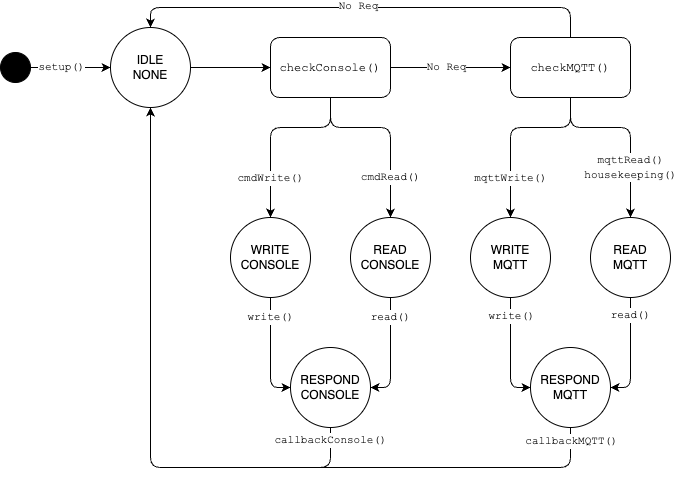
\includegraphics[width=.8\textwidth]{figs/2/FSM_IF.png}
    \caption[Finite State Machine for the IF Amplifier Control Loop]{Finite State Machine for the IF Amplifier Control Loop. Each state shows the current step in the process followed by the system that requested the action.}
    \label{chap2/fig:if_amp_fsm}
\end{figure}

For the Arduino control loop, we have implemented multiple ways to interact with the device using the \texttt{if\_amp} library.
For flight, we will be using the MQTT protocol to send messages to the Arduino to set the attenuation values and read the current attenuation values.
For testing, we have implemented both a simple serial interface. 
A web interface was also developed to control the attenuators using a web browser but was later removed to save on memory. 
Including the web interface adds additional static memory usage to the Arduino Nano Every in the form of large HTML strings.

The structure for the Arduino control loop is a fininte state machine that keeps track of the current request and which system requested it.
Figure \ref{chap2/fig:if_amp_fsm} shows the state diagram for the finite state machine.

The system starts with \texttt{setup()} which initliaizes all of the hardware interfaces and sets our initial state to \texttt{IDLE}.
Within \texttt{setup()}, we start our serial interface and initialize the I$^2$C bus.
Because of a hardware issue on the Printed Circuit Board (PCB), the \texttt{Wire} library needs to be patched to include timeouts on the I$^2$C bus.
This is because of a hardware issue where the Arduino has power but the rest of the system is off.
In this scenario, there is a floating voltage on the I$^2$C bus that causes the \texttt{Wire} library to hang indefinitely.
The patched \texttt{Wire} library has a new \texttt{setTimoout()} method that sets a timeout for the I$^2$C bus to prevent this from happening.

After setting up serial and I$^2$C, teh system sets up our Ethernet and MQTT connections.
For Ethernet, we are using the W5500 Ethernet shield from Wiznet \cite{w5500}.
This shield is connected to the Arduino using SPI and enables us to connect the Arduino to the rest of the readout network. 
To setup the networking, we give the Arduino a unique MAC address and a static IP address.
On ASTHROS, we have two of these systems so we provide them with addresses based on their hardcoded ID. 
In the case that the Arduino is not connected to the network, the system will continue to run but will only accept messages from the serial interface.
After setting up the Ethernet connection, we setup a client to connect to the MQTT broker.
This client takes the IP address of the broker and the port to connect to and attaches a callback function to handle incoming messages.
We then attempt a connection to the broker through the client using the name of our device and an account on our RabbitMQ server setup for handling MQTT requests.
Once connected, we subscribe to the \texttt{mqtt/comm/<ID>} topic where \texttt{<ID>} is the ID of the Arduino.
While AMQP and MQTT are different protocols, RabbitMQ has a plugin to handle MQTT messages and route them to the correct AMQP exchange.
By deafult messages published via MQTT are sent to the \texttt{amq.topic} exchange with the MQTT topic as the routing key, replacing the forward slashes with periods.
At the end of \texttt{setup()}, we initialize all of the attenuators to 31.75 dB and set the state to \texttt{IDLE}.

The \texttt{loop()} function is the main function that runs the finite state machine.
On top of the state and system variables, we have array buffers for \textt{addr}, \texttt{attn}, and \texttt{status} to store the address, attenuation value, and status of the current function call. 
There is also a flag for \texttt{single} that is used to indicuate if the current call is for a single channel or all channels.

In the \texttt{IDLE} state, we begin by checking if there is a message available on the serial interface. 
Using the \texttt{StaticSerialCommands} library, we can parse messages and call the appropriate callback function. 
Available commands are \texttt{w <addr> <attn>}, \texttt{wa <attn>}, \texttt{r <addr>}, and \texttt{ra} for writing and reading a single channel or all channels.
These commands do not actually execute the function but instead set the state to \texttt{WRITE} or \texttt{READ} with the appropriate address, attenuation value, and single flag.
We also set the system to \texttt{CONSOLE} to indicate that the serial interface requested the action.
In the case of a single channel operation, the first index of \texttt{addr} and \texttt{attn} are used. 
If the command is not recognized, an error message is sent back to the serial interface and we stay in the \texttt{IDLE} state.

If there are no commands waiting in the buffer and we are connected to the MQTT broker, we check for incoming messages.
If there is a message, we parse the message and set the state to \texttt{WRITE} or \texttt{READ} with the appropriate address, attenuation value, and single flag.
Messages from the MQTT broker are JSON strings with a \texttt{cmd} key that specifies the command and \texttt{addr} and \texttt{attn} keys that specify the address and attenuation value.
Additionally, we record the \texttt{routing\_ID} of the message in order to respond directly to the sender.
MQTT does not support direct addressing so we workaround this by sending a message to the topic exchange with the \texttt{routing\_ID} as the route. 
Whomever sends the request will need to subscribe to the \texttt{mqtt/comm/<routing\_ID>} topic to receive the response.

In the \texttt{READ} state, we call the \texttt{read()} command which begins a read operation on the Arduino. 
\texttt{read()} iterates over either all of the channels or just the first index and calls \texttt{single\_read()}.
The \texttt{single\_read()} function calls the \texttt{set\_attn()} function from the \texttt{if\_amp} library with the address and a pointer to the attenuation value.
We then store the status of the \texttt{set\_attn()} call in the corresponding index of \texttt{status}.
There is an error offset parameter that is used to add an offset to the status in case of errors.
This is used later in \texttt{single\_write()} to differenate between an error in writing and reading back the value. 
After reading all of the specified channels, we set the state to \texttt{RESPOND}.

In the \texttt{WRITE} state, we call the \texttt{write()} command which begins a write operation on the Arduino.
\texttt{write()} iterates over either all of the channels or just the first index and calls \texttt{single\_write()}.
\texttt{single\_write()} calls the \texttt{set\_attn()} function from the \texttt{if\_amp} library with the address and the attenuation value and saves the status. 
If the status is nonzero, we set the corresponding index in the attenuation buffer to -1 to indicate an error.
If not, we perform a \texttt{single\_read()} with an offset of 100 to indicate any errors in reading back the value came from the read operation. 

After either a read or write operation, the system ends up in the \texttt{RESPOND} state.
In this state, we check the system variable to see who requested the operation.
If the system is \texttt{CONSOLE}, we print out the status, attenuation, and address of either the single channel or all channels.
If the system is \texttt{MQTT}, we package the status, attenuation, and address into a JSON string and publish to the MQTT broker with the \texttt{mqtt/comm/<routing\_ID>} topic.
In either case, after sending the response, we clear the three buffers and set our state back to \texttt{IDLE}.

The firmware also has a few extra features to help configure the system.
The console also accepts an \texttt{mqtt} command that enables or disables the MQTT interface.
This is useful as, if the system is not connected to the network, the MQTT interface will continually try to connect and fail.
At a predefeined interval, the system will publish a message to the \texttt{mqtt/comm/<ID>} topic with the status of the system.
This is integrated into our state machine while checking for MQTT message by comparing the last time we published a status message with the current clock time and setting the state to \texttt{READ} and system to \texttt{MQTT} if the time has elapsed.
This read will read all channels and have an additional flag, \texttt{mqttStatus} that is checked in the \texttt{RESPOND} state to publish the status message to the MQTT broker with the \texttt{mqtt/comm/<ID>} topic instead of the routing ID.

There are also some quriks to the system that we attempt to mitigate in the firmware.
In addition to the I$^2$C bus issue, there is a hardware issue where the Ethernet shield will not initialize properly if the IF slices are powered on before the Arduino. 
In this case, we have a \texttt{pulseReset()} function that pulses the reset pin on the Ethernet shield to reset the shield and attempt to initialize the connection.
This occurs because power will leak through the SPI bus and partially power the shield.
When the system is fully on, the shield has an incorrect reference voltage and will not initialize properly during \texttt{setup()}.
\section{Housekeeping}

\section{Central Command}